\section{Grundlagen}
\begin{frame}
Hauptbefehle:
\begin{itemize}
%	\item <1->init
%	\note<1>{den Aktuellen Ordner zu einem Git Repository machen}
	\item <2->add
		\note<2>{Dateien/Änderungen zu einem aktuelle commit hinzufügen}
	\item <3->commit
		\note<3>[item]{Commits sind eingetragene Änderungen}
		\note<3>[item]{Diese Einträge sollten immer einen Titel haben der die Änderungen beschreiben}
		\note<3>[item]{Dabei sollte man eine Struktur einhalten, mehr dazu später.}
		\note<3>[item]{Vorsicht: Nach dem eine Änderung commited wurde ist sie noch nicht im Master Projekt zu finden. }
		\note<3>[item]{Dafür müssen die Änderungen...(push)}
	\item <4->push
		\note<4>[item]{Push leitet Vorgang ein, temporären Änderungen einzutragen}
	\item <5->pull
		\note<5>[item]{Pull wird zum kopieren des aktuellen Zustandes des Masterprojektes benutzt}
		\note<5>[item]{Alle gepushden Änderungen werden kopiert}
	\item <6->branch
		\note[item]<6>{Erstellung eines parallelen Stranges eines Projektes}
		\note[item]<6>{Master Branch besteht immer}
		\note[item]<6>{Man kann auf beiden Branches normal weiter arbeiten}
		\note[item]<6>{Bsp.: longtime Support alter Software und neue Version}
	\item <7->merge
		\note[item]<7>{Zusammenführen von branches}
		\note<7>[item]{Kann automatisch passieren}
		\note<7>[item]{Gleiche Passagen müssen per Hand gemacht werden}
\end{itemize}
\end{frame}

	\newcommand\commit[2][gray]{\node[commit,fill=#1,#1] (#2) {}; \node at (#2) {\small\strut};}
	\newcommand\commentm[2]{\node [clabel, outer sep=3em] at (#1) {#2}}
	\newcommand\commentb[2]{\node [clabel, outer sep=2.07em] at (#1) {#2}}
	\newcommand\commento[2]{\node [clabel, outer sep=1.17em] at (#1) {#2}}
	\newcommand\ghost[1]{\coordinate (#1);}
	\newcommand\connect[3][gray]{\path (#2) [draw=#1, line width=.18em] to[out=-90,in=90] (#3);}
\begin{frame}[fragile]
	\begin{tikzpicture}	
	\tikzstyle{commit}=[draw,circle,inner sep=0pt,minimum size=5pt]
	\tikzstyle{clabel}=[right]
	\tikzstyle{every path}=[draw]
	\matrix [column sep={.9em,between origins},row sep=\lineskip]
	{
	\commit{m1} & & \\
	& \commit[htwblue]{b1} & \\
	& \commit[htwblue]{b2} & \\
	\commit{m2} & \ghost{branch-o} & \\
	& & \commit[htworange]{o1} \\
	& \commit[htwblue]{b3} & \\
	\commit{m3} & & \ghost{merge-o} \\
	\commit{m4} & & \\
	\commit{m5} & & \\
	};
	% verbindungen:
	\connect[htworange]{branch-o}{o1};
	\connect[htworange]{o1}{merge-o};
	\connect[htworange]{merge-o}{m4};
	\connect[htwblue]{m1}{b1};
	\connect[htwblue]{b1}{b2};
	\connect[htwblue]{b2}{b3};
	\connect[htwblue]{b3}{m3};
	\connect[gray, shorten <= -10]{m1}{m2};
	\connect{m2}{m3};
	\connect{m3}{m4};
	\connect[gray, shorten >= -10]{m4}{m5};
	
	\commentm{m1}{{\visible<1->{\textcolor{htwgrey}{Master} Projekt (Master branch)}}};
	\commentb{b1}{{\visible<2->{\textcolor{htwblue}{Lukas} erstellt branch von \textcolor{htwgrey}{Master}}}};
	\commentb{b2}{{\visible<3->{commit von \textcolor{htwblue}{Lukas}}}};
%	\commentm{m2}{{\visible<4->{}}};
	\commento{o1}{{\visible<4->{\textcolor{htworange}{Johanna} erstellt branch von \textcolor{htwblue}{Lukas}}}};
%	\commentb{b3}{{\visible<6->{}}};
	\commentm{m3}{{\visible<5->{\textcolor{htwgrey}{Master} merged seinen branch mit \textcolor{htwblue}{Lukas} branch}}};
	\commentm{m4}{{\visible<6->{\textcolor{htwgrey}{Master} merged seinen branch mit \textcolor{htworange}{Johannas} branch}}};
%	\commentm{m5}{{\visible<9->{}}};
	\end{tikzpicture}
	%
\includegraphics[scale=0.3]{Bilder/git_graph1}
	\note{Beispiel eines git Projektverlaufes}
	\note<1>[item]{Aktuellste eingetragene Zustände eines Projektes}
	\note<2>[item]{Branches tragen nicht den Namen des Erstellers}
	\note<2>[item]{Es braucht nicht jeder Nutzer einen eigenen Branch}
\end{frame}


%\begin{frame}
%	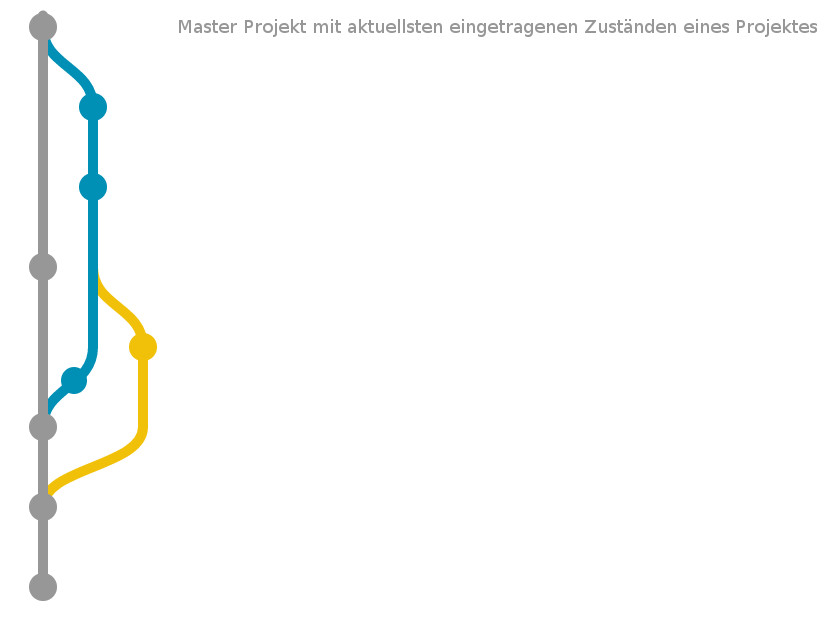
\includegraphics[scale=0.3]{Bilder/git_graph2}
%	\note{Graue Linie: Master Projekt mit aktuellsten Änderungen. Alles geht zurück auf das Master Projekt. Es existiert immer nur ein Projekt mit dem interagiert wird.}
%\end{frame}
%\begin{frame}
%	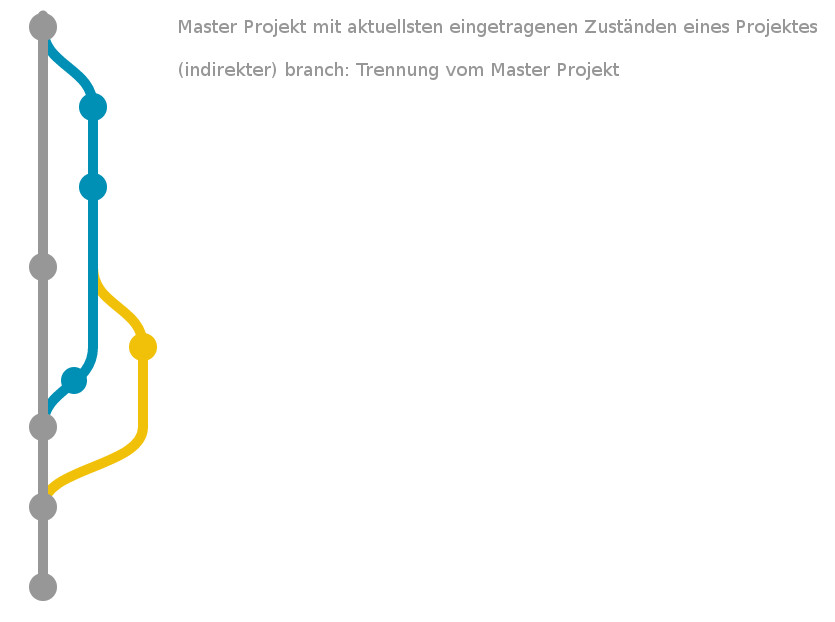
\includegraphics[scale=0.3]{Bilder/git_graph3}
%	\note{Bei einer Änderung wird ein indirekter Branch einer Projektes erstellt, wie zum Beispiel bei einem...(commit)}
%\end{frame}
%\begin{frame}
%	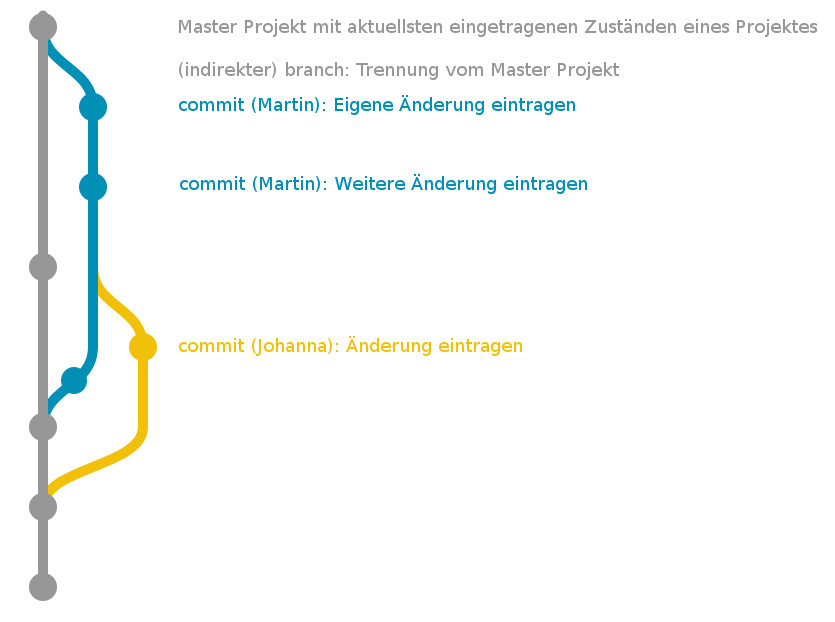
\includegraphics[scale=0.3]{Bilder/git_graph4}
%\end{frame}
%\begin{frame}
%	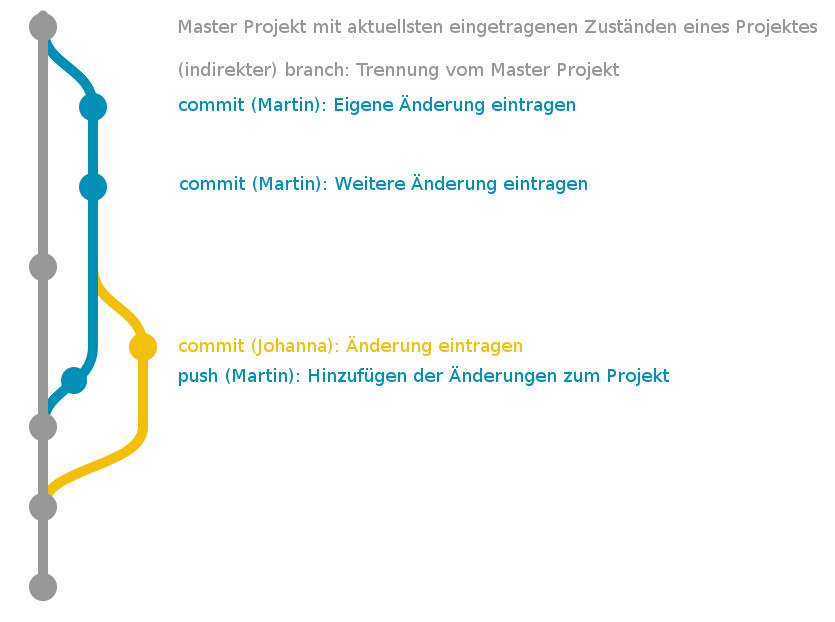
\includegraphics[scale=0.3]{Bilder/git_graph5}
%\end{frame}
%\begin{frame}
%	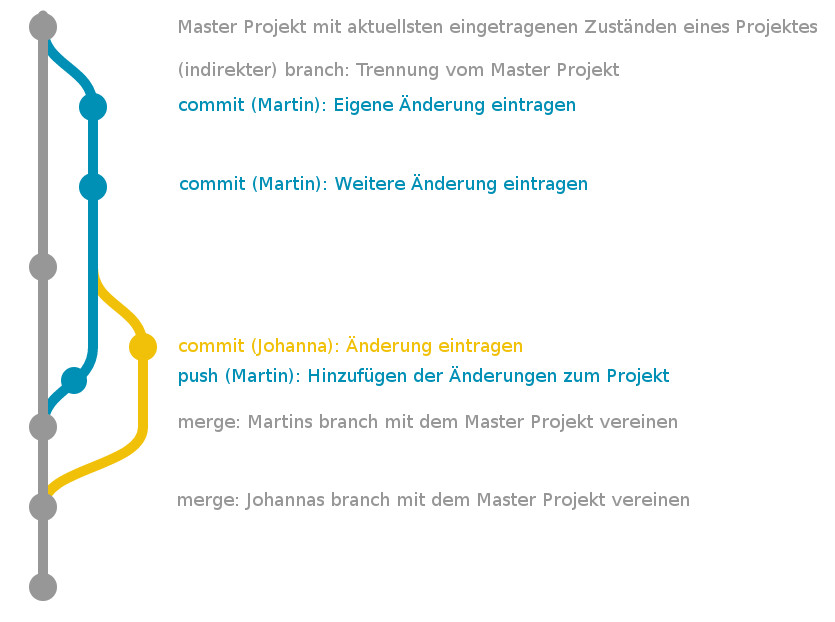
\includegraphics[scale=0.3]{Bilder/git_graph6}
%	\note{Beim zusammenführen der Dateien zum Master Projekt wird ein merge gemacht, damit sind nun die Änderungen in das Master Projekt eingetragen worden}
%\end{frame}
%\subsection{Details}
%\begin{frame}
%Hier noch ein paar Details.
%\end{frame}